\documentclass[conference]{IEEEtran}
\IEEEoverridecommandlockouts
% The preceding line is only needed to identify funding in the first footnote. If that is unneeded, please comment it out.
\usepackage{cite}
\usepackage{amsmath,amssymb,amsfonts}
\usepackage{algorithmic}
\usepackage[spanish]{babel}
\usepackage[utf8]{inputenc}
\usepackage{graphicx}
\usepackage{textcomp}
\usepackage{xcolor}
\usepackage{hyperref}
\usepackage{multirow}
\usepackage{float}
\usepackage{subcaption}
\usepackage{listings}
\usepackage{color}
\definecolor{mygreen}{rgb}{0,0.6,0}
\definecolor{mygray}{rgb}{0.5,0.5,0.5}
\definecolor{mymauve}{rgb}{0.58,0,0.82}

\def\BibTeX{{\rm B\kern-.05em{\sc i\kern-.025em b}\kern-.08em
    T\kern-.1667em\lower.7ex\hbox{E}\kern-.125emX}}
\lstset{
  basicstyle=\footnotesize,        % the size of the fonts that are used for the code
  breakatwhitespace=false,         % sets if automatic breaks should only happen at whitespace
  breaklines=true,                 % sets automatic line breaking
  captionpos=b,                    % sets the caption-position to bottom
  commentstyle=\color{mygreen},    % comment style
  deletekeywords={...},            % if you want to delete keywords from the given language
  escapeinside={\%*}{*)},          % if you want to add LaTeX within your code
  extendedchars=true,              % lets you use non-ASCII characters; for 8-bits encodings only, does not work with UTF-8
  keepspaces=true,                 % keeps spaces in text, useful for keeping indentation of code (possibly needs columns=flexible)
  keywordstyle=\color{blue},       % keyword style
  language=C,                 % the language of the code
  morekeywords={*,...},
  emph={alt_up_char_buffer_string,IORD,IOWR},
  emphstyle=\color{red},
  %numbers=left,                    % where to put the line-numbers; possible values are (none, left, right)
  %numbersep=2pt,                   % how far the line-numbers are from the code
  %numberstyle=\tiny\color{mygray},            % if you want to add more keywords to the set
  rulecolor=\color{black},         % if not set, the frame-color may be changed on line-breaks within not-black text (e.g. comments (green here))
  showspaces=false,                % show spaces everywhere adding particular underscores; it overrides 'showstringspaces'
  showstringspaces=false,          % underline spaces within strings only
  showtabs=false,                  % show tabs within strings adding particular underscores
  stepnumber=2,                    % the step between two line-numbers. If it's 1, each line will be numbered
  tabsize=1,
  frame=trBL,	              % sets default tabsize to 2 spaces
  basicstyle=\scriptsize\ttfamily
}

\begin{document}

\title{
Diseño e Implementación de un servidor de base de datos utilizando la FPGA Terasic DE10-Standard \\
}

\author{\IEEEauthorblockN{\textbf{Lino Ontano}}
\IEEEauthorblockA{	\textit{Telemática}
\\Guayaquil - Ecuador \\
lontano@espol.edu.ec
}
\and
\IEEEauthorblockN{\textbf{Jocelyn Miranda}}
\IEEEauthorblockA{	\textit{Telemática}
\\Guayaquil - Ecuador \\
jocammir@espol.edu.ec
}
}

\maketitle

\begin{abstract}
	Diseño e implementación de un sistema que realiza el monitoreo a una base de datos implementada en el sistema operativo Linux del Hard Processor System (HPS) de la FPGA Terasic DE10-Standard y es mostrada por pantalla utilizando protocolo VGA.
\end{abstract}
\begin{IEEEkeywords}
FPGA, HPS, VGA
\end{IEEEkeywords}

\section{Introducción}\label{sec:int}
El presente proyecto se basa en el diseño y la implementación de un sistema embebido que realice monitoreo a una base de datos. El servidor de la base de datos es implementado en el Hard Processor System (HPS) de la FPGA Terasic DE-10 Standard, la cuál es manejada vía Putty SSH conectada a una red local. La FPGA es la encargada de realizar las consultas por medio de sus periféricos de entrada al HPS el cual ejecuta scripts que devuelven valores y escribe esos resultados en memoria para que la FPGA lea y muestre el resultado por pantalla por medio de su puerto VGA. El proyecto consta de tres etapas:
\begin{enumerate}
  \item Montar el servidor de la base de datos en el HPS, habilitar el acceso vía SSH y configurar las interfaces de red para el acceso en la red local. La imagen del sistema operativo es proporcionada por la tarjeta desde el sitio web de Terasic.
  \item Diseñar e implementar la arquitectura de la FPGA donde el procesador Nios II enviará datos para ser mostrados por medio del VGA. Además de proporcionar acceso a los periféricos de entrada, para nuestro caso, habilitar acceso a los \textit{switches} que puedan ser leídos por el procesador y acceso a la \textit{On-Chip Memory} de la FPGA, para leer los valores que serán enviados por el HPS en la siguiente etapa.
  \item Finalmente, la arquitectura desarrollada deberá ser levantada por el HPS, para ello, se utilizará el proyecto de demostración Control Panel QT\footnote{El proyecto Control Panel QT se lo puede encontrar en el CD proporcionado por la tarjeta; cuenta con licencia en ciertos bloques, los cuales no son utilizados y lo demás es utilizado exclusivamente con fines educativos.} y se modificará dicha arquitectura y se agregará los bloques que requerimos. Se utiliza ese proyecto ya que contiene lo necesario para el correcto funcionamiento del HPS junto a la FPGA.
\end{enumerate}
\section{Metodología}
\subsection{Hardware}
\subsubsection*{Tarjeta de desarrollo DE10-Standard}
\begin{figure}[h]
	\centerline{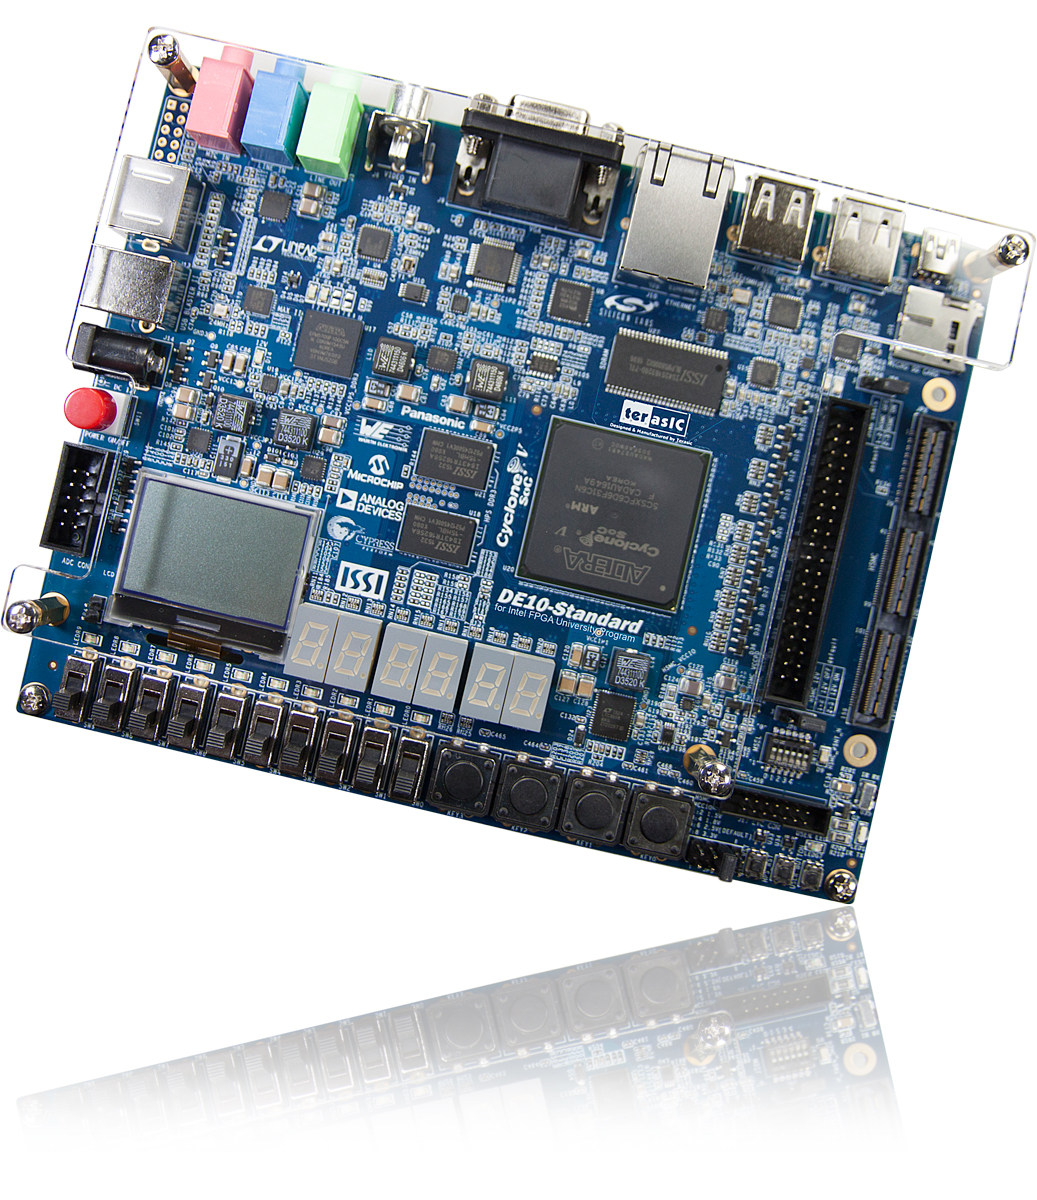
\includegraphics[width=0.25\textwidth]{img/at01.jpg}}
	\caption{Tarjeta DE10-Standard.}
	\label{fig:hw01}
\end{figure}
El kit de desarrollo DE10-Standard presenta una robusta plataforma de diseño de hardware construida alrededor del Intel System-on-Chip (SoC) FPGA, que combina los últimos núcleos incorporados de doble núcleo Cortex-A9 con una lógica programable líder en la industria para una máxima flexibilidad de diseño. Los usuarios ahora pueden aprovechar la potencia de una reconfigurabilidad tremenda combinada con un sistema de procesador de bajo rendimiento y alto rendimiento. El SoC de Altera integra un sistema de procesador duro (HPS) basado en ARM que consiste en un procesador, periféricos e interfaces de memoria vinculados sin problemas con el tejido FPGA utilizando una red troncal de interconexión de gran ancho de banda.\\
La placa DE10-Standard tiene muchas características que permiten a los usuarios implementar una amplia gama de circuitos diseñados, desde circuitos simples hasta varios proyectos multimedia.\\
\textsc{FPGA}
\begin{itemize}
	\item Intel Cyclone V SX SoC—5CSXFC6D6F31C6N
	\item Dispositivo de configuración serial - EPCS128
	\item USB-Blaster II onboard for programming; JTAG Mode
	\item 64MB SDRAM (16-bit data bus)
	\item 4 botoneras
	\item 10 switches
	\item 10 LEDs
	\item 6 pantallas de 7 segmentos
	\item Cuatro fuentes de reloj de 50MHz del generador de reloj
	\item 24-bit CD-quality audio CODEC con línea de entrada, línea de salida y jack de entrada de micrófono.
	\item VGA DAC con conector VGA de salida
	\item Decoder de TV y conector de entrada de TV
	\item PS/2 mouse/conector de teclado
	\item IR receptor y emisor.
	\item Un HSMC con configuración I/O standard 1.5/1.8/2.5/2.3
	\item Una expansión de 40 pines con protección de diodos.
	\item A/D convertidor, 4 pines SPI interfaz con FPGA
\end{itemize}\vspace{2mm}
\textsc{ARM-Based Hard Processor System\textbf{ (HPS)} }
\begin{itemize}
	\item 925 MHz Dual-core ARM Cortex-A9 MPCore processor
	\item 1GB DDR3 SDRAM (32-bit data bus)
	\item 1 Gigabit Ethernet PHY con conector RJ45
	\item 2 puertos USB Host, conector USB normal tipo-A
	\item Socket para tarjeta Micro SD
	\item Acelerómetro (interfaz 12C + interrupt)
	\item UART a USB, USB mini-B conector
	\item botón reset \textit{warm} y botón reset \textit{cold}
	\item Un botón de usuario y un LED de usuario
	\item LTC 2x7 cabecera de expansión
	\item 128x64 puntos de módulo LCD con blacklight
\end{itemize}
\subsubsection*{Device Tree Blob}
Para el correcto funcionamiento del hardware de la FPGA con el sistema operativo de la HPS requerimos una estructura que permita acceder y usar esos componentes. Un \textit{Device  Blob} es una estructura de datos que describe los componentes de hardware de un dispositivo en particular para que así el \textit{kernel} del sistema operativo pueda usarlo y manejar esos componentes. Se requerirá generar el archivo .dtb para que exista el puente entre el HPS y la FPGA.
\begin{figure}[h]
	\centerline{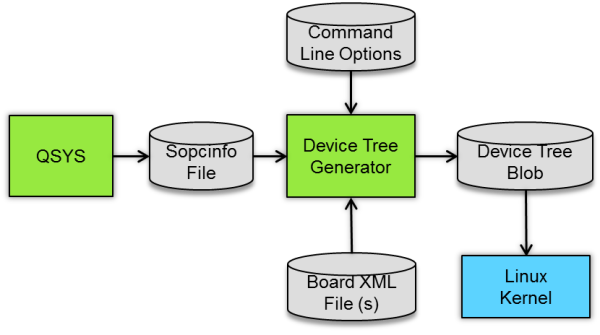
\includegraphics[width=0.4\textwidth]{img/dtb.png}}
	\caption{Generador del Device Tree.}
	\label{fig:hw02}
\end{figure}

\subsection{Arquitectura}
En la FPGA se requiere tener acceso al periférico de los \textit{switches}, tener un \textit{On-Chip Memory} y un procesador Nios II como arquitectura básica. Para poder mostrar las consultas de la base, requerimos mostrar texto por medio del VGA. Para lograr aquello, utilizamos un bloque denominado \textit{Character Buffer}, que consta con librerías para poder ser manipulado desde el procesador y mostrar las líneas que queramos. Ese Character Buffer requiere transformar su salida a una frecuencia manejable para el VGA \textit{Controller}, por tanto se utiliza un \textit{Dual Clock Buffer}, que baja la frecuencia de salida del \textit{Character Buffer} a 25MHz. El VGA \textit{Controller} que se conecta al VGA DAC para mostrar por pantalla. Para el correcto funcionamiento del HPS se añade a la arquitectura de la FPGA un procesador ARM, y varios componentes que utiliza el HPS obtenido del proyecto de demostración antes mencionado.\\
En el HPS debe estar montado la base de datos en la microSD que contiene la imagen del sistema operativo, además de los archivos de la arquitectura de la FPGA antes creada para acceder, desde el kernel, a los periféricos FPGA por medio del \textit{bridge}. Todo lo antes mencionado está resumido en la figura \ref{fig:arq01}.\\
Para lograr la arquitectura, el Qsys\footnote{Qsys es una herramienta de integración del sistema en el software Quartus® Prime que ahorra tiempo y esfuerzo en el proceso de diseño de FPGA.} requiere utilizar los siguientes componentes:
\begin{itemize}
  \item Arria V/Cyclone V Hard Processor System
  \item Nios II Processor
  \item Clock Source
  \item Avalon-MM Pipeline Bridge
  \item JTAG UART
  \item System ID Peripheral
  \item Interval Timer
  \item On-Chip Memory (RAM or ROM)
  \item PIO (Parallel I/O) x3(Leds, Switches y Keys)
  \item SPI (3 Wire Serial)
  \item Altera PLL
  \item Character Buffer for VGA display
  \item Dual-Clock FIFO
  \item VGA Controller
  \item Contador (IP propio)
  \item Divisor Clock (IP propio)
\end{itemize}
\begin{figure}[h]
	\centerline{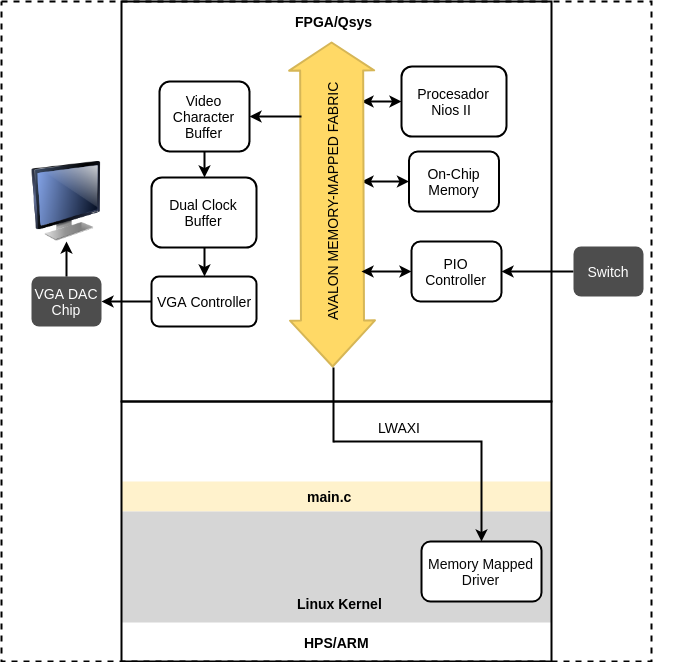
\includegraphics[width=0.5\textwidth]{img/arq.png}}
	\caption{\textit{Diagrama de bloques de la arquitectura}}
	\label{fig:arq01}
\end{figure}
Existen dos componentes IP propias que muestran el tiempo de ejecución de las consultas por medio de un reloj de 1Hz. Los demás bloques se pueden obtener directamente del catálogo IP del Qsys.

\begin{figure}[h]
	\centerline{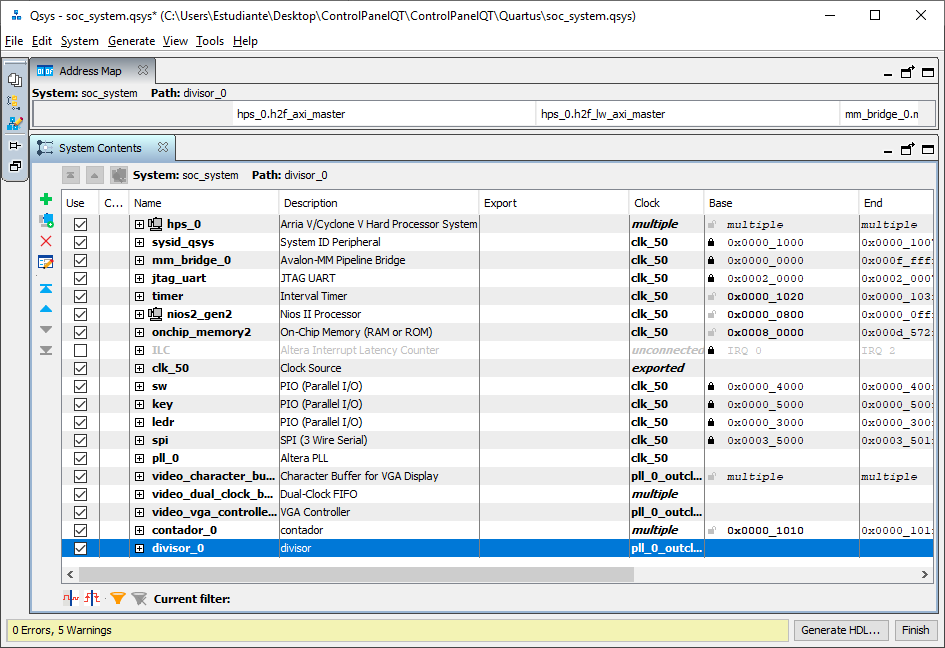
\includegraphics[width=0.4\textwidth]{img/qsys02.png}}
	\caption{\textit{Ventana Qsys con arquitectura}}
	\label{fig:qsys01}
\end{figure}

\subsection{Software}
Existen tres programas en C que se ejecutan en nuestro proyecto:
\begin{figure}[h]
    \begin{subfigure}[h]{0.5\textwidth}
       \centerline{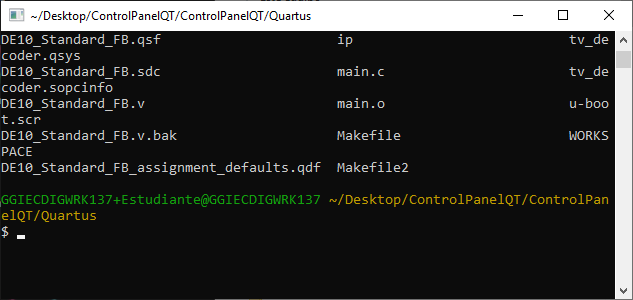
\includegraphics[width=0.6\textwidth]{img/eds01.png}}
       \caption{\textit{Ventana Soc EDS}}

    \end{subfigure}\\
    \begin{subfigure}[h]{0.5\textwidth}
      \centerline{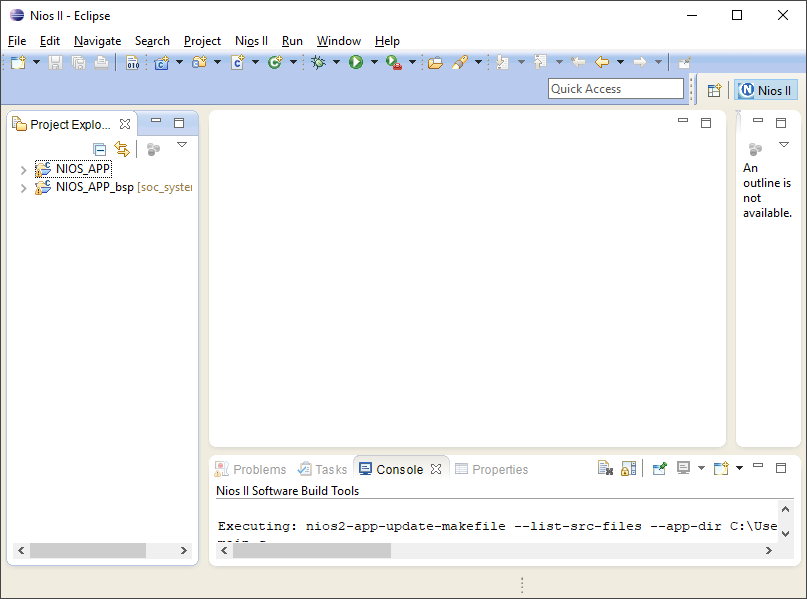
\includegraphics[width=0.6\textwidth]{img/eclipse.png}}
      \caption{\textit{Ventana Eclipse}}

    \end{subfigure}
    \caption{\textit{Herramientas utilizadas}}
\label{fig:sw01}
\end{figure}
\begin{itemize}
  \item Un programa que se ejecuta en la \textbf{FPGA} por medio del Nios II, que se encarga de leer en memoria y mostrar por pantalla lo que nos mande el HPS, interactúa con los \textit{switches} para decidir cuando mostrar la consulta por pantalla.
  \item Dos programa que se ejecuta en el \textbf{HPS}. Uno realiza la consulta a la base de datos y el resultado lo guarda en un archivo de texto, y el segundo se encarga de leer esos archivos y guardarlos en la memoria \textit{On-Chip} de la FPGA, además interactúa con los \textit{switches} para decidir en que momento realizar una determinada consulta y almacenarla.
\end{itemize}
El programa de la FPGA se carga en el Nios II utilizando la herramienta \textit{Nios II Software Build Tools for Eclipse}, mientras que en el HPS se lo realiza localmente con la herramienta \textit{SoC EDS Command Shell} y se pasa el ejecutable por protocolo SSH.
\subsubsection*{Programa FPGA}
El programa en C que se realizó en la FPGA utiliza la siguiente librería:
\lstinputlisting[language = C, firstline=4, lastline=4]{script/main.c}
que permite comunicarse con el \textit{Character Buffer} para imprimir datos a la pantalla. \\
Para cada consulta, la FPGA si se activa el \textit{switch} SW9, mostrará por pantalla utilizando los siguientes métodos:
\lstinputlisting[language = C, firstline=33, lastline=45]{script/main.c}
Se observa que lee la información de la \textit{On-Chip} por medio de la función {\footnotesize\texttt{IORD}}. Y muestra las diferentes líneas con el método {\footnotesize\texttt{alt\_up\_char\_buffer\_string}}, que se le manda la cadena de caracteres a mostrar con su ubicación por medio de unas coordenadas en x,y.

\subsubsection*{Programa HPS}
El programa en C que se realizó en el HPS es generado por un makefile que importa las librerías requeridas para el proyecto:
\lstinputlisting[language = C, firstline=1, lastline=11]{script/mainHPS.c}
El script lee los valores de los switches para determinar que combinación ha sido accionada, de acuerdo a eso dependerá del valor que guarde de la consulta, que es generada por un script de bash que ejecuta otro C que contiene el acceso a la base y la sentencia a consultar, y se lo lee por medio de una función que accede al archivo de texto generado con el resultado de la consulta.
\lstinputlisting[language = C, firstline=47, lastline=61]{script/mainHPS.c}

\section{Análisis de Resultados}\label{sec:resul}
El programa en HPS consiguió acceder a los periféricos de la FPGA, mostrando sus valores y los cambios cuando eran accionados. El programa en la FPGA, imprime los valores establecidos de acuerdo al accionar del \textit{switch} SW9 y la lectura de la memoria y su impresión en pantalla por medio del protocolo VGA. \\
El script que hace la consulta a la base, devolvían los valores mostrados en la tabla y son guardados en un archivo de texto. El programa en HPS es capaz de leer los valores del archivo resultado de la consulta, y almacenado en memoria para ser mostrado por pantalla por la FPGA.\\
\begin{figure}[h]
	\centerline{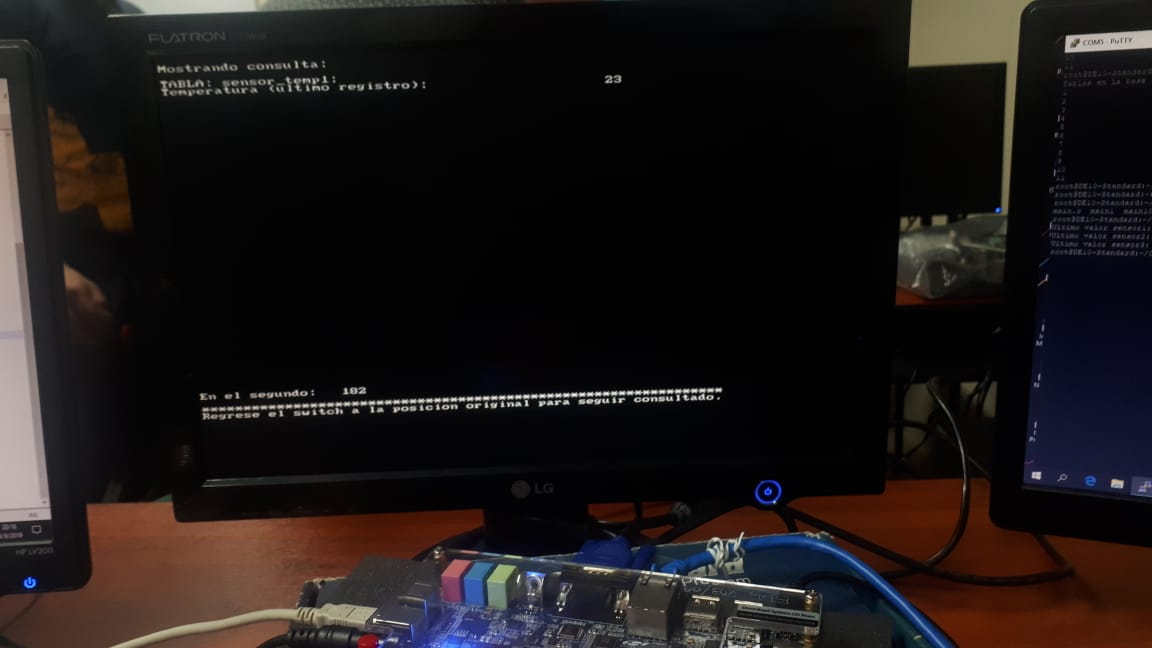
\includegraphics[width=0.4\textwidth]{img/res01.jpeg}}
	\caption{\textit{Salida por pantalla por parte de la FPGA}}
	\label{fig:qsys01}
\end{figure}
Existen inconvenientes al querer acceder o almacenar a más valores de la memoria compartida, ya que las direcciones no coinciden entre el HPS y la FPGA en su totalidad. Se debe a que la arquitectura difiere un poco del archivo \textit{header} del script del HPS; por lo que para lograr varias consultas de varios datos a la vez, se necesita corregir y generar un \textit{header} de acuerdo a la nueva arquitectura. De esta forma tenemos más datos para enviarle a la FPGA por parte del HPS y de esa manera volver más dinámica la consulta.

\section{Conclusiones}
\begin{itemize}
	\item Se implementó un sistema embebido que accede a base de datos por medio de un \textit{bridge} entre una arquitectura FPGA y HPS.
	\item Se requirió generar un \textit{Device Tree} para realizar el puente por medio de comandos no disponibles en el manual.
  \item Las consultas a la base de datos requiere más manejo de memoria para poder realizar múltiples consultas a la vez.
  \item Es importante entender como se guarda la información en la memoria \textit{On-Chip} para poder acceder a ella y no generar mal funcionamiento de la FPGA.
\end{itemize}


\begin{thebibliography}{00}
\bibitem{b1} Roberto Fernandez Molanes, Filipe Salgado, Jose Farina, Juan Rodriguez, ``Characterization of FPGA-Master ARM Communication Delays in Cyclone V Devices '', 2015.
\bibitem{b2} Terasic, ``DE10'Standard QT Control Panel Manual'', 2017.
\bibitem{b3} Terasic, ``DE10'Standard User Manual'', 2017.
\bibitem{b3} GitHub: robertofem, ``Angstrom 2013.12'', \url{https://github.com/robertofem/CycloneVSoC-examples/tree/master/SD-operating-system/Angstrom-v2013.12}
 2013.
\bibitem{b3} Altera Corporation, ``Cyclone V Device Handbook'', 2014.
\end{thebibliography}

\end{document}
